% Options for packages loaded elsewhere
\PassOptionsToPackage{unicode}{hyperref}
\PassOptionsToPackage{hyphens}{url}
\PassOptionsToPackage{dvipsnames,svgnames,x11names}{xcolor}
%
\documentclass[
  authoryear,
  preprint]{elsarticle}

\usepackage{amsmath,amssymb}
\usepackage{iftex}
\ifPDFTeX
  \usepackage[T1]{fontenc}
  \usepackage[utf8]{inputenc}
  \usepackage{textcomp} % provide euro and other symbols
\else % if luatex or xetex
  \usepackage{unicode-math}
  \defaultfontfeatures{Scale=MatchLowercase}
  \defaultfontfeatures[\rmfamily]{Ligatures=TeX,Scale=1}
\fi
\usepackage{lmodern}
\ifPDFTeX\else  
    % xetex/luatex font selection
\fi
% Use upquote if available, for straight quotes in verbatim environments
\IfFileExists{upquote.sty}{\usepackage{upquote}}{}
\IfFileExists{microtype.sty}{% use microtype if available
  \usepackage[]{microtype}
  \UseMicrotypeSet[protrusion]{basicmath} % disable protrusion for tt fonts
}{}
\makeatletter
\@ifundefined{KOMAClassName}{% if non-KOMA class
  \IfFileExists{parskip.sty}{%
    \usepackage{parskip}
  }{% else
    \setlength{\parindent}{0pt}
    \setlength{\parskip}{6pt plus 2pt minus 1pt}}
}{% if KOMA class
  \KOMAoptions{parskip=half}}
\makeatother
\usepackage{xcolor}
\setlength{\emergencystretch}{3em} % prevent overfull lines
\setcounter{secnumdepth}{5}
% Make \paragraph and \subparagraph free-standing
\makeatletter
\ifx\paragraph\undefined\else
  \let\oldparagraph\paragraph
  \renewcommand{\paragraph}{
    \@ifstar
      \xxxParagraphStar
      \xxxParagraphNoStar
  }
  \newcommand{\xxxParagraphStar}[1]{\oldparagraph*{#1}\mbox{}}
  \newcommand{\xxxParagraphNoStar}[1]{\oldparagraph{#1}\mbox{}}
\fi
\ifx\subparagraph\undefined\else
  \let\oldsubparagraph\subparagraph
  \renewcommand{\subparagraph}{
    \@ifstar
      \xxxSubParagraphStar
      \xxxSubParagraphNoStar
  }
  \newcommand{\xxxSubParagraphStar}[1]{\oldsubparagraph*{#1}\mbox{}}
  \newcommand{\xxxSubParagraphNoStar}[1]{\oldsubparagraph{#1}\mbox{}}
\fi
\makeatother


\providecommand{\tightlist}{%
  \setlength{\itemsep}{0pt}\setlength{\parskip}{0pt}}\usepackage{longtable,booktabs,array}
\usepackage{calc} % for calculating minipage widths
% Correct order of tables after \paragraph or \subparagraph
\usepackage{etoolbox}
\makeatletter
\patchcmd\longtable{\par}{\if@noskipsec\mbox{}\fi\par}{}{}
\makeatother
% Allow footnotes in longtable head/foot
\IfFileExists{footnotehyper.sty}{\usepackage{footnotehyper}}{\usepackage{footnote}}
\makesavenoteenv{longtable}
\usepackage{graphicx}
\makeatletter
\newsavebox\pandoc@box
\newcommand*\pandocbounded[1]{% scales image to fit in text height/width
  \sbox\pandoc@box{#1}%
  \Gscale@div\@tempa{\textheight}{\dimexpr\ht\pandoc@box+\dp\pandoc@box\relax}%
  \Gscale@div\@tempb{\linewidth}{\wd\pandoc@box}%
  \ifdim\@tempb\p@<\@tempa\p@\let\@tempa\@tempb\fi% select the smaller of both
  \ifdim\@tempa\p@<\p@\scalebox{\@tempa}{\usebox\pandoc@box}%
  \else\usebox{\pandoc@box}%
  \fi%
}
% Set default figure placement to htbp
\def\fps@figure{htbp}
\makeatother

\usepackage{booktabs}
\usepackage{caption}
\usepackage{longtable}
\usepackage{colortbl}
\usepackage{array}
\usepackage{anyfontsize}
\usepackage{multirow}
\makeatletter
\@ifpackageloaded{caption}{}{\usepackage{caption}}
\AtBeginDocument{%
\ifdefined\contentsname
  \renewcommand*\contentsname{Table of contents}
\else
  \newcommand\contentsname{Table of contents}
\fi
\ifdefined\listfigurename
  \renewcommand*\listfigurename{List of Figures}
\else
  \newcommand\listfigurename{List of Figures}
\fi
\ifdefined\listtablename
  \renewcommand*\listtablename{List of Tables}
\else
  \newcommand\listtablename{List of Tables}
\fi
\ifdefined\figurename
  \renewcommand*\figurename{Figure}
\else
  \newcommand\figurename{Figure}
\fi
\ifdefined\tablename
  \renewcommand*\tablename{Table}
\else
  \newcommand\tablename{Table}
\fi
}
\@ifpackageloaded{float}{}{\usepackage{float}}
\floatstyle{ruled}
\@ifundefined{c@chapter}{\newfloat{codelisting}{h}{lop}}{\newfloat{codelisting}{h}{lop}[chapter]}
\floatname{codelisting}{Listing}
\newcommand*\listoflistings{\listof{codelisting}{List of Listings}}
\makeatother
\makeatletter
\makeatother
\makeatletter
\@ifpackageloaded{caption}{}{\usepackage{caption}}
\@ifpackageloaded{subcaption}{}{\usepackage{subcaption}}
\makeatother
\journal{Open Quaternary}

\usepackage[]{natbib}
\bibliographystyle{elsarticle-harv}
\usepackage{bookmark}

\IfFileExists{xurl.sty}{\usepackage{xurl}}{} % add URL line breaks if available
\urlstyle{same} % disable monospaced font for URLs
\hypersetup{
  pdftitle={Biogeography of crop progenitors and wild plant resources in the terminal Pleistocene and Early Holocene of West Asia, 14.7--8.3 ka},
  pdfauthor={Joe Roe; Amaia Arranz-Otaegui},
  colorlinks=true,
  linkcolor={blue},
  filecolor={Maroon},
  citecolor={Blue},
  urlcolor={Blue},
  pdfcreator={LaTeX via pandoc}}


\setlength{\parindent}{6pt}
\begin{document}

\begin{frontmatter}
\title{Biogeography of crop progenitors and wild plant resources in the
terminal Pleistocene and Early Holocene of West Asia, 14.7--8.3 ka}
\author[1,2]{Joe Roe%
\corref{cor1}%
}
 \ead{joeroe@hey.com} 
\author[3]{Amaia Arranz-Otaegui%
%
}


\affiliation[1]{organization={University of
Bern},country={Switzerland},countrysep={,},postcodesep={}}
\affiliation[2]{organization={University of
Copenhagen},country={Denmark},countrysep={,},postcodesep={}}
\affiliation[3]{organization={University of the Basque
Country},country={Spain},countrysep={,},postcodesep={}}

\cortext[cor1]{Corresponding author}


        
\begin{abstract}
This paper presents the first continuous, spatially-explicit
reconstructions of the palaeodistributions of 81 plant species found
regularly in association with early agricultural archaeological sites in
West Asia, including the progenitors of the first crops. We used machine
learning to train an ecological niche model of each species based on its
present-day distribution in relation to climate and environmental
variables. Predictions of the potential ranges of these species at key
stages of the Pleistocene--Holocene transition could then be derived
from these models using downsampled data from palaeoclimate simulations.
The models predict significant reductions and/or shifts in species
ranges in the terminal Pleistocene and Early Holocene compared to
present conditions. Many species that are found throughout the region's
`hilly flanks' today are indicated to have much more restricted
distributions centered on the Levant, Cyprus and Western Anatolia. In
addition, overall ranges shrunk by an average of c.~25\% from the
terminal Pleistocene to the Early Holocene. Modelled ranges do not
reliably predict the observed occurrence of specific species at
archaeological sites, however {[}\ldots{]} The regional ubiquity of
species in the archaeological record is {[}not{]} correlated with the
predicted size of its range and the diversity of archaeobotanical
assemblages is {[}not{]} correlated with the predicted diversity of its
environs. This indicates that trends in taxonomic composition of the
archaeobotanical record is {[}not{]} likely to have been influenced by
environmental change and species turnover, in addition to human economic
choices.
\end{abstract}





\end{frontmatter}
    

\begin{itemize}
\tightlist
\item[$\boxtimes$]
  Stop modelling
\item[$\square$]
  First draft:

  \begin{itemize}
  \tightlist
  \item[$\boxtimes$]
    Introduction
  \item[$\square$]
    Background

    \begin{itemize}
    \tightlist
    \item[$\square$]
      Biogeography
    \item[$\boxtimes$]
      ENM
    \end{itemize}
  \item[$\boxtimes$]
    Methods \& Materials
  \item[$\boxtimes$]
    Results
  \item[$\square$]
    Discussion

    \begin{itemize}
    \tightlist
    \item[$\boxtimes$]
      General trends
    \item[$\square$]
      Case studies
    \item[$\boxtimes$]
      Comparison with archaeobot
    \end{itemize}
  \item[$\square$]
    Conclusion
  \end{itemize}
\item[$\square$]
  Figures

  \begin{itemize}
  \tightlist
  \item[$\boxtimes$]
    fig-region
  \item[$\boxtimes$]
    fig-occ
  \item[$\square$]
    tbl-occ-count (needs pdf cleanup)
  \item[$\square$]
    tbl-predictors
  \item[$\square$]
    tbl-model-metrics
  \end{itemize}
\item[$\square$]
  Outstanding TODOs
\item[$\square$]
  Add missing references
\item[$\square$]
  Copyedit
\item[$\boxtimes$]
  Appendix with all hindcast predictions (HTML?)
\item[$\square$]
  Clean up package code
\item[$\square$]
  Final proofread
\end{itemize}

\section{Introduction}\label{introduction}

The Pleistocene--Holocene transition in West Asia marked a turning point
in global environmental history, as humans brought the first plants
under cultivation and began modifying surrounding ecosystems to support
their own subsistence. West Asia is part of the native range of a
remarkable number of domesticable plant species, including wild
relatives of wheat, barley, peas, lentils, and other crops of global
importance \citep{cite}. Even before the end of the Ice Age, these
species supported uniquely dense and complex Late Epipalaeolithic
(15--11.7 ka) societies based on intensive foraging \citep{cite} and
eventually pre-domestication cultivation \citep{cite}. As they were
brought under domestication in the Pre-Pottery Neolithic period
(11.7--8.5 ka), the world's first agriculture was shaped by the
ecosystems from which it emerged and was embedded in.

Decades of research in archaeobotany and zooarchaeology have
reconstructed the subsistence economies of Late Epipalaeolithic and
Neolithic sites in great detail \citep{cites}. Together with studies of
charcoal \citep{cite}, pollen \citep{cite}, soil \citep{cite}, and a
variety of palaeoclimate archives \citep{JonesEtAl2019}, they also tell
us much about the environments surrounding these settlements. However,
each of these sources of evidence is subject to the wide variety of
taphonomic and recovery biases that are inherent in any direct record of
the past. They are also, by definition, records of the (human)
environment at particular times and places. Interpolating these
snapshots to give a holistic picture of the regional ecologies is not
straightforward -- to date, it has tended to rely on non-explicit,
inductive modelling. The majority are also filtered through human
action, producing a mixed single that makes it difficult to disentangle
anthropic effects from the background of environmental change in this
period of rapid climatic alteration.

In this paper we present a complementary, deductive approach based on
ecological niche modelling. Rather than inferring environmental
conditions from preserved physical evidence, we predict the ranges of
individual species relevant to human subsistence based on a model of
their current environmental niche and simulations of past palaeoclimate.
Though hypothetical, this gives us an independent line of evidence on
past ecologies that is independent of the environmental archaeological
and palaeoclimatic records. Our computational approach is also readily
scaled up, allowing us to model spatially-explicit palaeodistributions
for a large number of species, for the whole region, under multiple past
climatologies.

\section{Background}\label{background}

\begin{itemize}
\tightlist
\item
  The transition to agriculture in West Asia was\ldots{}
\end{itemize}

\subsection{Biogeography and agricultural
origins}\label{biogeography-and-agricultural-origins}

\begin{itemize}
\tightlist
\item
  Has always been important in study of agricultural origins

  \begin{itemize}
  \tightlist
  \item
    Historically: Vavilov, Pumpelly \& Childe
  \item
    Genetic studies tell us origin points, but not ranges
  \end{itemize}
\item
  Important to e.g.

  \begin{itemize}
  \tightlist
  \item
    Distinguish environmental from potentially anthropogenic change
    \citep{MartinEtAl2016, MartinEtAl2025}
  \item
    Reconstruct sequences of domestication \citep{YeomansEtAl2017}
  \end{itemize}
\item
  Epipal./Neo. plant-based economies were diverse

  \begin{itemize}
  \tightlist
  \item
    More than the ``founder crops'';
  \item
    More than food
  \item
    (In archaebot., not all intentionally collected)
  \item
    Geographically and temporally diverse
  \item
    \ldots so we model lots of species!
  \end{itemize}
\item
  Regional ecological reconstructions generally rely on the `expert
  interpolation' (or what do they call it with isoscapes?) method

  \begin{itemize}
  \tightlist
  \item
    See CSEAS (AEA-prep) presentation
  \item
    Figure: comparisons
  \end{itemize}
\end{itemize}

\subsection{Ecological niche modelling in
archaeology}\label{ecological-niche-modelling-in-archaeology}

Ecological niche modelling (ENM) or species distribution modelling (SDM)
is widely used by ecologists to predict the geographic range of a
species based on a set of environmental predictors. Essentially, it
involves combining records of where an organism has been observed with
environmental data (climate, topography, etc.) for those locations to
model the range of environmental values at which that species -- its
environmental niche. This model can then be used to predict the range of
the organism in question either in the same or a different environment.
\citet{CITE} suggests reserving the term `species distribution
modelling' for when the method is used to recover the verifiable range
of a species in a real and existing environment, and using `ecological
niche modelling' as the broader term covering hypothetical or predictive
applications -- a convention we follow here when referring to predictive
or `hindcast' models of past ranges. Within this overarching framework,
ecological niche modelling encompasses a wide range of applications and
a variety of potential environmental predictors, modelling approaches,
and methodologies, which we will not attempt to review here.

Ecological niche modelling has long been of interest to archaeologists
as both a means of exploring the biological niche of humans and for
reconstructing the past environments they inhabited
\citep{DavidPollyEronen2011, FranklinEtAl2015}. In the first sense, it
has been used most extensively to model the range of humans and other
hominin species
\citep[e.g.][]{BenitoEtAl2017, YousefiEtAl2020, BanksEtAl2021, YaworskyEtAl2024a, YaworskyEtAl2024b, GuranEtAl2024},
especially in the Palaeolithic. This overlaps with what archaeologists
usually call generically `predictive modelling'
\citep{VerhagenWhitley2020}---more precisely `site distribution
modelling'---which is essentially the same approach as (and often
borrows methodologies from) ecological niche modelling but applied to
the occurrence of archaeological sites. Here what is modelled is not
strictly a biological niche alone, but also aspects of human geography,
taphonomy, and archaeological visibility. These applications can be
distinguihed from `palaeoecological niche modelling', where the object
of model remains, as in ecology, a non-human biological niche.

\citet{FranklinEtAl2015} review palaeoecological niche modelling and
advocate for its greater adoption in environmental archaeology. In an
early application to West Asia, \citet{ConollyEtAl2012} used the
occurrence of wild and domestic \emph{Bos} remains at prehistoric
archaeological sites to map the evolving niche of cattle over the
Pleistocene--Holocene transition. It has been used to model the
availability of fauna exploited by humans at wider scales
\citep[e.g.][]{deAndresHerreroEtAl2018, YaworskyEtAl2023} and, in a West
Asian context, of foraged plant resources in the landscape around the
Neolithic site of XX \citep{CollinsEtAl2018}. Modelling the spread of
crops has been another significant archaeological application
\citep{CremaEtAl}.

In the majority of studies to date (palaeo)ecological niche modelling
has been applied to archaeological data in an `inductive' fashion,
i.e.~faunal and botanical remains from ancient sites are used as the
occurrence dataset for training a model using either past or present
environmental data. However, both the zooarchaeological and
archaeobotanical records are sparse and subject to a complex array of
depositional, taphonomic and recovery biases factors that , many of
which are not fully understood and/or cannot be corrected for. This
means that while the archaeological attestation of the presence of a
species might generally be relied upon, it is highly unlikely that its
absence is representative of true past distributions.

The alternative approach is to train the model using contemporary
occurrence and environmental data and then use palaeoenvironmental data
to `hindcast' its predictions backwards in time. Like
\citet{FranklinEtAl2015}, we view the hindcasting approach as more
promising, because training datasets for both occurrences and
environment are far more readily available, complete and reliable for
the present than the past. There is some scepticism in the ecological
niche modelling literature about the ability of such models to make
accurate predictions in unknown environments (like the past)
\citep{CITES}, but here the hindcasting approach also presents an
opportunity: it reserves archaeological occurrence data as an
independent dataset that can be used to assess the retrodictive
performance of the model. This possibily was suggested by
\citet{FranklinEtAl2015} but to our knowledge our study represents the
first attempt to actually do so.

The major practical limitation of the hindcasting approach is that it
relies on spatially explicit, high resolution palaeoenvironmental
surfaces with continuous coverage of the region and periods of interest.
Until recently, this has not been widely available for most
applications, which is perhaps why only a minority of studies use it
\citep[cf.][]{YaworskyEtAl2023}. In this study, we are able to take
advantage of the increasing availability of high resolution, global
palaeoclimate data derived from simulation experiments with general
circulation models of climate
\citep{BrownEtAl2018, BrownEtAl2020, KargerEtAl2023}.

\section{Data and model}\label{data-and-model}

\begin{figure}

\centering{

\pandocbounded{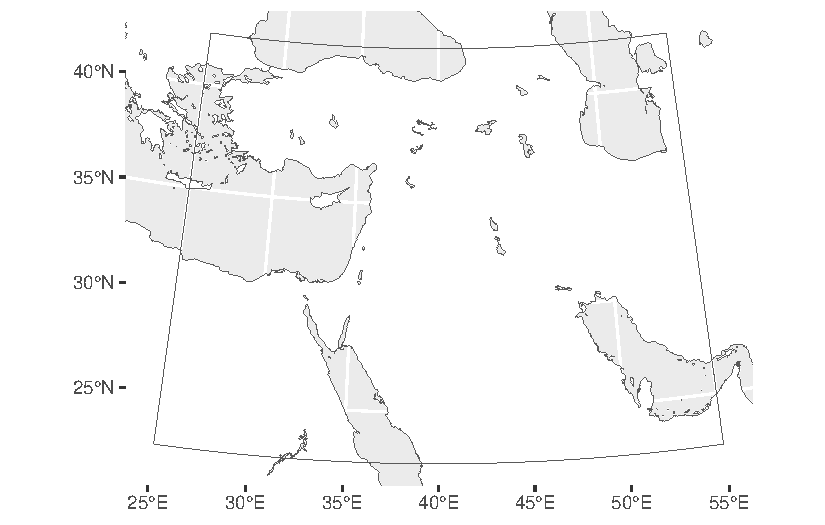
\includegraphics[keepaspectratio]{paper_files/figure-pdf/fig-region-1.pdf}}

}

\caption{\label{fig-region}Late Epipalaeolithic \& Pre-Pottery Neolithic
archaeological sites used to generate modelled flora}

\end{figure}%

The aim of our study was to model the biogeography of species relevant
to human subsistence economies in West Asia (excluding the Southern
Arabian peninsula, see Figure~\ref{fig-region}) during the
archaeological Late Epipalaeolithic (15--11.7 ka) and Pre-Pottery
Neolithic (11.7--8.3 ka) periods. Our starting point was a list of 96
taxa (Table~\ref{tbl-taxa}) comprising the identifiable species observed
at at least two Late Epipalaeolithic/Pre-Pottery Neolithic sites,
according to our previous study of the regional archaeobotanical data
\citep{ArranzOtaeguiRoe2023}. This was based on dataset of 117
assemblages collated from three previously published regional
archaeobotanical databases: ADEMNES \citep{ADEMNES}, ORIGINS
\citep{ORIGINS}, and COMPAG \citep{COMPAG}. We did not attempt to
distinguish between the source of the remains; archaeobotanical
assemblages are subject to a variety of preservational and recovery
biases, so by no means were all the species on our list consumed or even
deliberately collected by people. However, we assume that there presence
at a site of human settlement at least implies that they were part of
the wider ecosystem that supported habitation there.

Taxonomic names were resolved to the canonical form specified in the
GBIF Backbone Taxonomy \citep{GBIFSecretariat2023}. So for example
occurrences for \emph{Bolboschoenus maritimus} also include those
recorded under the older nomenclature \emph{Scirpus maritimus} (see
Table~\ref{tbl-taxa}). Domestic species meeting our inclusion criteria
were substituted with their wild progenitor(s), where different.

\subsection{Occurrence data}\label{occurrence-data}

Georeferenced occurrence data for West Asia was obtained from the Global
Biodiversity Information Facility (GBIF) using via its application
programming interface and the R package `rgbif'
\citep{ChamberlainBoettiger2017, rgbif}. GBIF was cleaned to removed
fossil occurrences, recorded absences, and records with missing,
imprecise (\textgreater1 km uncertainty), or invalid coordinates.
Although niche models have reasonable predictive power even with small
training samples
\citep{StockwellPeterson2002, HernandezEtAl2006, WiszEtAl2008}, we
excluded 81 taxa with less than 50 usable occurrences, following
recommendations for niche models generally and Random Forest-based
models specifically \citep{StockwellPeterson2002, LuanEtAl2020}. We also
excluded one taxon (\emph{Avena sterilis}) with over 50,000 occurrences,
as this would have been computationally prohibitive and we were
uncertain what accounted for such a disproportionately high number of
records.

\begin{figure}

\centering{

\pandocbounded{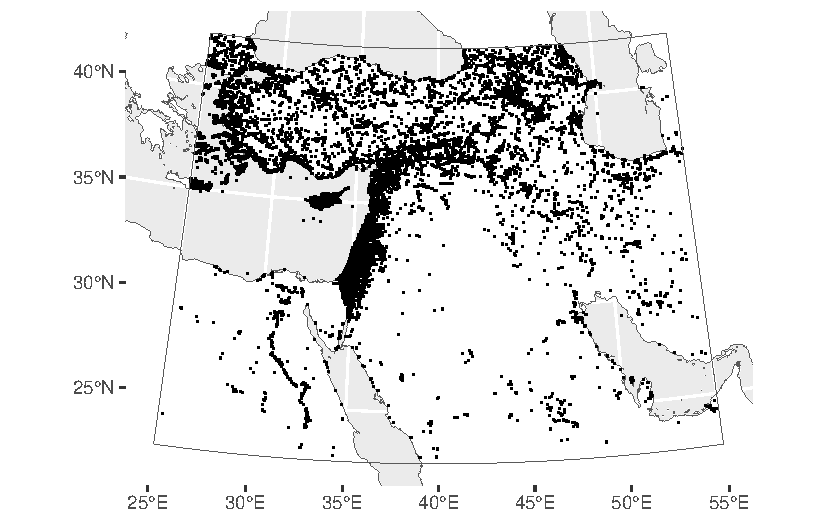
\includegraphics[keepaspectratio]{paper_files/figure-pdf/fig-occ-map-1.pdf}}

}

\caption{\label{fig-occ-map}Georeferenced occurrence records from West
Asia used to train models (N=78222}

\end{figure}%

Occurrence data only tells us where a species is present; there is
rarely definitive information on where the species is \emph{not} found.
We therefore need to generate random background points or
``pseudo-absences'' to feed to the model. There are several ways to do
this. We follow the advice of \citet{BarbetMassinEtAl2012} for
regression-based species distribution models and use a large (≈10000)
random sample of points, weighted equally against the presences in the
regression. \citet{ValaviEtAl2022} also recommend using a large
background sample for random forest models.

\subsection{Predictor data}\label{predictor-data}

We modelled the occurrence of species as a function of X spatial
predictor variables (Table~\ref{tbl-predictors}). These included:

\begin{itemize}
\tightlist
\item
  Sixteen `bioclimatic' variables derived from monthly temperature and
  precipitation values, following standard practice for species
  distribution models \citep{HijmansEtAl2005}. Contemporary bioclimatic
  predictor data for West Asia was extracted from the global CHELSA
  dataset \citep{KargerEtAl2017}, which predicts temperature and
  precipitation from downscaled general circulation model output at 1 km
  resolution.
\end{itemize}

\begin{itemize}
\tightlist
\item
  Terrain aspect and slope, which at high resolution perform well as
  proxies for solar radiation when modelling plant occurrence
  \citep{AustinVanNiel2011, LeempoelEtAl2015}; and the topographic
  wetness index (TWI), which serves as a proxy for soil moisture and is
  particularly important in modelling arid environments
  \citep{KopeckyCizkova2010, CamposEtAl2016, DiVirgilioEtAl2018}. All
  three were derived from the SRTM15+ digital elevation model using
  algorithms from WhiteboxTools \citep{Lindsay2016}.
\end{itemize}

\begin{itemize}
\tightlist
\item
  Edaphic data from SoilGrids \citep{HenglEtAl2014, HenglEtAl2017},
  which improves model performance for plants
  \citep{DubuisEtAl2013, ModEtAl2016, VelazcoEtAl2017}. Based on a
  recent assessment of the reliability of SoilGrids data for species
  distribution modelling \citep{MillerEtAl2024}, we used a subset of
  four variables relating to soil texture (clay, silt, sand) and pH at
  the surface (0-5 cm depth).
\end{itemize}

Predictor data was transformed to common equal-area projection and
resolution of 5 km.

\begin{table}

\caption{\label{tbl-climate-periods}}

\centering{

\fontsize{12.0pt}{14.4pt}\selectfont
\begin{tabular*}{\linewidth}{@{\extracolsep{\fill}}lr}
\toprule
Period & Age, ka \\ 
\midrule\addlinespace[2.5pt]
Bølling-Allerød (BA) & 14.7–12.9 \\ 
Younger Dryas (YDS) & 12.9–11.7 \\ 
Early Holocene (EH) & 11.7–8.3 \\ 
Current (CUR) & — \\ 
\bottomrule
\end{tabular*}

Palaeoclimatic periods used for hindcasting, after \citet{BrownEtAl2018}

}

\end{table}%

For hindcasting, we used reconstructed bioclimatic data for 3 key
periods (Table~\ref{tbl-climate-periods}) generated from downscaled
paleoclimate simulations from the HadCM3 general circulation model
\citep{BrownEtAl2018}. Terrain and soil predictors were held constant,
since reconstructions of these variables in the past are not available
at sufficient scale. It is not likely that either macroscale topography
or soil characteristics have altered significantly over the period of
time considered here, so we assume that this does not degrade model
performance, and may in fact benefit it by providing `anchoring'
predictors that are independent of climate change.

\subsection{Random Forest}\label{random-forest}

Ecological niche modelling is a classification problem that can be
approached with a wide range of statistical methods. A substantial
literature exists on the relatively performance of these approaches and
their respective parameterisations \citep[reviewed
in][]{ValaviEtAl2022}. Random Forest, a widely-used machine learning
algorithm, is amongst the best performing methods for presence-only
species distribution models, providing it is appropriately parameterised
to account for the class imbalance between presence and background
samples \citep{ValaviEtAl2021, ValaviEtAl2022}. For our application, it
also has the advantage of requiring little to no manual parameter tuning
to achieve good predictive results, which makes it easier to model a
larger numbers of taxa.

For each taxon we trained a classification model to predict occurrence
(presence or absence/background) based on our X predictor variables
(Table~\ref{tbl-predictors}). We used the Random Forest algorithm
implemented in the R package `ranger' \citep{WrightZiegler2017} and the
`tidymodels' \citep{tidymodels} framework for data preprocessing and
model selection. To avoid overfitting, we follow \citet{ValaviEtAl2021}
in their recommended hyperparameters and use of down-sampling to balance
presence and background samples. Models for each taxon were fit
independently, with redundant zero-variance predictors excluded, and
assessed based on balanced training (¾) and test (¼) partitions.

\section{Model assessment}\label{model-assessment}

We trained Random Forest models for 81 taxa using contemporary
occurrence data from GBIF, a random sample of background points, and the
predictor variables described in Table~\ref{tbl-predictors}.
Substituting the ``current'' climate predictors for those derived from
palaeoclimatic simulations \citep{BrownEtAl2018}, we could then generate
hindcast predictions for reconstructed past environments in 4 key
climate periods -- a total of 324 modelled palaeodistributions.
Predicted distributions for individual taxa are presented in the
appendix and accompanying material.

\begin{figure}

\centering{

\pandocbounded{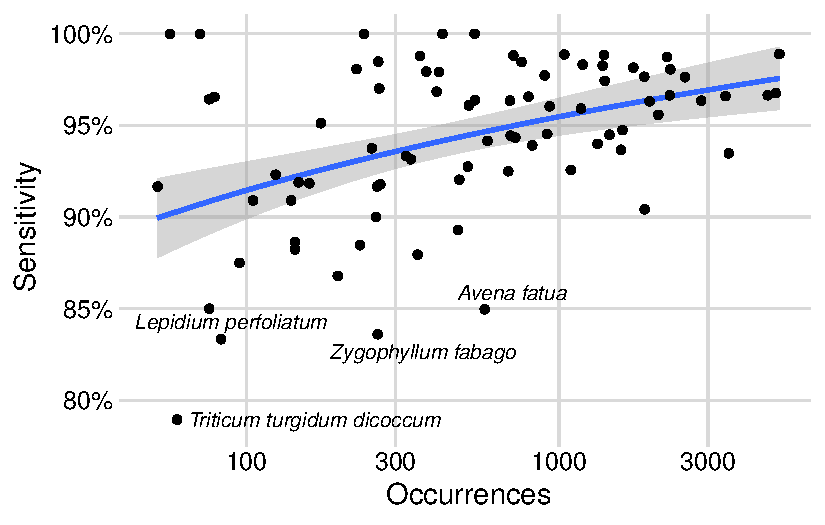
\includegraphics[keepaspectratio]{paper_files/figure-pdf/fig-model-sensitivity-vs-n_occ-1.pdf}}

}

\caption{\label{fig-model-sensitivity-vs-n_occ}Model sensitivity by
number of training occurrences}

\end{figure}%

We assessed the predictive performance of the fitted niche models in the
contemporary environment based on the reserved test partition. Model
accuracy (proportion of correctly classified presence and background
samples) ranged between 72\% and 99\%, with an average of 92\%.
Sensitivity (proportion of correctly classified presence samples) ranged
between 79\% and 100\%, with an average of 94\%. The area under the
models' receiver operating characteristic curves (ROC-AUC) was in the
range of 0.978±0.061 Model sensitivity is loosely correlated with the
number of occurrences available for training
(Figure~\ref{fig-model-sensitivity-vs-n_occ}), with the worst-performing
models all having less than 300 recorded occurrences: \emph{Avena
fatua}, \emph{Lepidium perfoliatum}, \emph{Triticum turgidum dicoccum},
and \emph{Zygophyllum fabago}. Test metrics and ROC curves for the
individual models are included in the appendix.

The ability of the hindcast models to predict the occurrence of specific
species at archaeological sites is significantly worse, with only 5\% of
presences in archaeobotanical assemblages successfully predicted.

\section{Discussion}\label{discussion}

\begingroup
\setlength\LTleft{0\linewidth}
\setlength\LTright{0\linewidth}\fontsize{8.2pt}{9.9pt}\selectfont

\begin{longtable}{@{\extracolsep{\fill}}lrrrrr}

\caption{\label{tbl-taxa}Summary of species modelled}

\tabularnewline

\toprule
 & \multicolumn{2}{c}{Occurrences} & \multicolumn{3}{c}{Model} \\ 
\cmidrule(lr){2-3} \cmidrule(lr){4-6}
Taxon & Archaeological & Present (GBIF) & Accuracy & ROC-AUC & Sensitivity \\ 
\midrule\addlinespace[2.5pt]
{\itshape Adonis dentata} & 2 & 715 & 0.99 & 1.00 & 0.99 \\ 
{\itshape Aegilops crassa} & 4 & 143 & 0.82 & 0.94 & 0.89 \\ 
{\itshape Aegilops speltoides} & — & 701 & 0.93 & 0.98 & 0.94 \\ 
{\itshape Aegilops tauschii} & — & 725 & 0.90 & 0.98 & 0.94 \\ 
{\itshape Aizoanthemopsis hispanica} & 4 & 515 & 0.98 & 0.99 & 0.96 \\ 
{\itshape Ammi majus} & 4 & 900 & 0.99 & 0.99 & 0.98 \\ 
{\itshape Androsace maxima} & 17 & 231 & 0.88 & 0.96 & 0.88 \\ 
{\itshape Arenaria serpyllifolia} & 3 & 139 & 0.85 & 0.94 & 0.91 \\ 
{\itshape Arnebia decumbens} & 21 & 324 & 0.94 & 0.98 & 0.93 \\ 
{\itshape Arnebia linearifolia} & 13 & 225 & 0.98 & 1.00 & 0.98 \\ 
{\itshape Asphodelus aestivus} & 2 & 76 & 0.96 & 0.97 & 0.96 \\ 
{\itshape Atriplex prostrata} & 4 & 266 & 0.97 & 1.00 & 0.97 \\ 
{\itshape Avena fatua} & 2 & 579 & 0.85 & 0.93 & 0.85 \\ 
{\itshape Bassia arabica} & 4 & 264 & 0.98 & 1.00 & 0.98 \\ 
{\itshape Bolboschoenus maritimus} & 29 & 1040 & 0.98 & 1.00 & 0.99 \\ 
{\itshape Brachypodium distachyon} & 5 & 2270 & 0.98 & 0.99 & 0.98 \\ 
{\itshape Bromus sterilis} & 3 & 759 & 0.96 & 1.00 & 0.98 \\ 
{\itshape Buglossoides arvensis} & 23 & 260 & 0.86 & 0.96 & 0.90 \\ 
{\itshape Buglossoides tenuiflora} & 26 & 252 & 0.96 & 0.99 & 0.94 \\ 
{\itshape Capparis spinosa} & 4 & 4938 & 0.97 & 0.99 & 0.97 \\ 
{\itshape Capsella bursa-pastoris} & 2 & 1329 & 0.94 & 0.99 & 0.94 \\ 
{\itshape Carex divisa} & 9 & 336 & 0.95 & 0.98 & 0.93 \\ 
{\itshape Ceratonia siliqua} & 2 & 5072 & 0.98 & 1.00 & 0.99 \\ 
{\itshape Chenopodium album} & 5 & 480 & 0.93 & 0.98 & 0.92 \\ 
{\itshape Cicer reticulatum} & 3 & 52 & 0.96 & 1.00 & 0.92 \\ 
{\itshape Citrullus colocynthis} & 4 & 475 & 0.89 & 0.95 & 0.89 \\ 
{\itshape Crithopsis delileana} & 3 & 406 & 0.97 & 0.99 & 0.97 \\ 
{\itshape Erodium ciconium} & 2 & 359 & 0.91 & 0.99 & 0.99 \\ 
{\itshape Ficus carica} & 8 & 3495 & 0.93 & 0.98 & 0.93 \\ 
{\itshape Fumaria densiflora} & 4 & 413 & 0.98 & 0.99 & 0.98 \\ 
{\itshape Gypsophila elegans} & 3 & 76 & 0.93 & 0.96 & 0.85 \\ 
{\itshape Gypsophila pilosa} & 5 & 173 & 0.93 & 0.99 & 0.95 \\ 
{\itshape Gypsophila vaccaria} & 8 & 511 & 0.96 & 0.99 & 0.93 \\ 
{\itshape Halothamnus hierochunticus} & 2 & 57 & 0.99 & 1.00 & 1.00 \\ 
{\itshape Helianthemum ledifolium} & 2 & 697 & 0.97 & 0.98 & 0.96 \\ 
{\itshape Helianthemum salicifolium} & 2 & 1400 & 0.98 & 0.99 & 0.97 \\ 
{\itshape Hordeum bulbosum} & 4 & 2850 & 0.97 & 0.99 & 0.96 \\ 
{\itshape Hordeum murinum} & 5 & 1949 & 0.95 & 0.99 & 0.96 \\ 
{\itshape Hordeum spontaneum} & 51 & 4656 & 0.96 & 0.99 & 0.97 \\ 
{\itshape Juglans regia} & 2 & 821 & 0.85 & 0.96 & 0.94 \\ 
{\itshape Lathyrus aphaca} & 4 & 2079 & 0.95 & 0.99 & 0.96 \\ 
{\itshape Lathyrus cicera} & 2 & 591 & 0.90 & 0.98 & 0.94 \\ 
{\itshape Lathyrus oleraceus} & 6 & 1580 & 0.88 & 0.97 & 0.94 \\ 
{\itshape Lathyrus sativus} & 4 & 196 & 0.80 & 0.94 & 0.87 \\ 
{\itshape Lepidium perfoliatum} & 3 & 83 & 0.80 & 0.92 & 0.83 \\ 
{\itshape Linum bienne} & 9 & 376 & 0.96 & 1.00 & 0.98 \\ 
{\itshape Lolium rigidum} & 5 & 2529 & 0.98 & 1.00 & 0.98 \\ 
{\itshape Lolium temulentum} & 3 & 159 & 0.93 & 0.95 & 0.92 \\ 
{\itshape Medicago astroites} & 15 & 143 & 0.90 & 0.97 & 0.88 \\ 
{\itshape Medicago minima} & 2 & 1379 & 0.92 & 0.99 & 0.98 \\ 
{\itshape Medicago radiata} & 20 & 799 & 0.93 & 0.99 & 0.97 \\ 
{\itshape Moltkia coerulea} & 2 & 71 & 0.86 & 0.99 & 1.00 \\ 
{\itshape Neotorularia torulosa} & 2 & 539 & 0.98 & 0.99 & 0.96 \\ 
{\itshape Peganum harmala} & 2 & 917 & 0.91 & 0.98 & 0.95 \\ 
{\itshape Phalaris paradoxa} & 3 & 1191 & 0.99 & 0.99 & 0.98 \\ 
{\itshape Phragmites australis} & 4 & 3412 & 0.97 & 0.99 & 0.97 \\ 
{\itshape Pistacia atlantica} & 6 & 1874 & 0.98 & 1.00 & 0.98 \\ 
{\itshape Plantago lagopus} & 2 & 1730 & 0.98 & 1.00 & 0.98 \\ 
{\itshape Poa bulbosa} & 5 & 1880 & 0.95 & 0.98 & 0.90 \\ 
{\itshape Prosopis farcta} & 5 & 2263 & 0.97 & 1.00 & 0.97 \\ 
{\itshape Quercus ithaburensis} & 2 & 2216 & 0.98 & 1.00 & 0.99 \\ 
{\itshape Rumex pulcher} & 6 & 1394 & 0.98 & 1.00 & 0.99 \\ 
{\itshape Salsola kali} & 6 & 537 & 0.98 & 1.00 & 1.00 \\ 
{\itshape Salvia absconditiflora} & 3 & 105 & 0.92 & 0.99 & 0.91 \\ 
{\itshape Secale cereale} & 4 & 268 & 0.79 & 0.95 & 0.92 \\ 
{\itshape Secale strictum} & 3 & 124 & 0.74 & 0.96 & 0.92 \\ 
{\itshape Stipa dregeana} & 2 & 79 & 0.93 & 0.99 & 0.97 \\ 
{\itshape Suaeda fruticosa} & 3 & 238 & 0.99 & 1.00 & 1.00 \\ 
{\itshape Taeniatherum caput-medusae} & 4 & 262 & 0.82 & 0.96 & 0.92 \\ 
{\itshape Tribulus terrestris} & 2 & 1091 & 0.91 & 0.97 & 0.93 \\ 
{\itshape Triticum aestivum compactum} & 2 & 147 & 0.80 & 0.96 & 0.92 \\ 
{\itshape Triticum durum} & 3 & 95 & 0.90 & 0.94 & 0.88 \\ 
{\itshape Triticum monococcum aegilopoides} & 36 & 1176 & 0.88 & 0.98 & 0.96 \\ 
{\itshape Triticum turgidum dicoccum} & 47 & 60 & 0.72 & 0.85 & 0.79 \\ 
{\itshape Triticum urartu} & — & 424 & 0.93 & 1.00 & 1.00 \\ 
{\itshape Verbena officinalis} & 3 & 934 & 0.95 & 0.99 & 0.96 \\ 
{\itshape Vicia ervilia} & 26 & 688 & 0.88 & 0.97 & 0.93 \\ 
{\itshape Vicia faba} & 7 & 1597 & 0.91 & 0.98 & 0.95 \\ 
{\itshape Vicia narbonensis} & 3 & 1451 & 0.93 & 0.98 & 0.94 \\ 
{\itshape Vicia orientalis} & 14 & 353 & 0.84 & 0.95 & 0.88 \\ 
{\itshape Zygophyllum fabago} & 3 & 263 & 0.89 & 0.95 & 0.84 \\ 
\bottomrule

\end{longtable}

\endgroup

\subsection{Reduction in range sizes over the Pleistocene/Holocene
boundary}\label{reduction-in-range-sizes-over-the-pleistoceneholocene-boundary}

\begin{figure}

\centering{

\pandocbounded{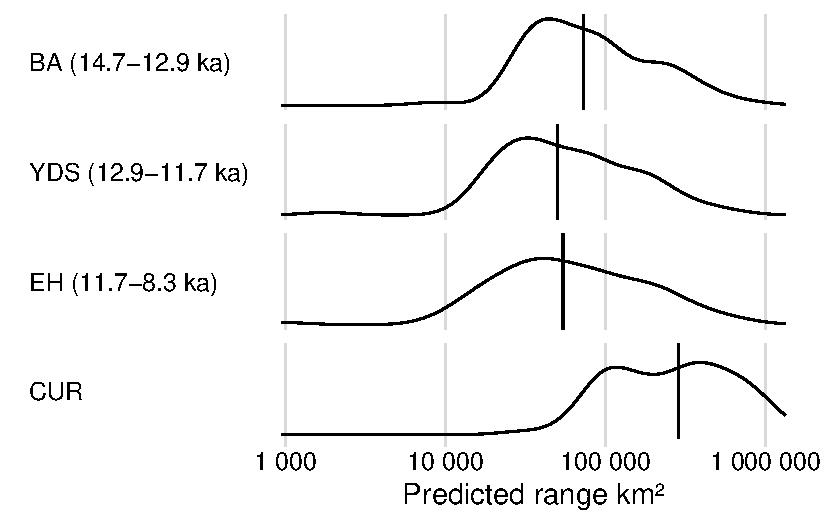
\includegraphics[keepaspectratio]{paper_files/figure-pdf/fig-pred-range-density-1.pdf}}

}

\caption{\label{fig-pred-range-density}Distribution of predicted species
ranges by period. Dashed lines indicate the median range.}

\end{figure}%

Our reconstructed palaeodistributions (shown in full in the appendix)
indicate that the majority of species have experienced a significant
reduction and/or shift in their ranges since the Early Holocene. 75 of
81 species have reduced ranges; 65 of more than 10\% or more. Though the
magnitude of the reduction from prehistory to the present likely
reflects a degree of overfitting in the model (discussed further below),
fluctuations in modelled range size between the Bølling-Allerød
(14.7--12.9 ka), Younger Dryas (12.9--11.7 ka), and Early Holocene
(11.7--8.3 ka) are more directly comparable
\textbf{?@fig-range-density}. The average range of modelled species was
25\% in the Early Holocene compared to the Bølling--Allerød, and 32\%
during the Younger Dryas (i.e.~ranges recovered slightly between the
Younger Dryas and Early Holocene). This perhaps indicates that although
this period is considered one of climatatic amelioration globally
\citep{JonesEtAl2019}, the colder conditions of the Pleistocene may have
supported more extensive plant-based economies in West Asia
specifically.

\begin{figure}

\centering{

\pandocbounded{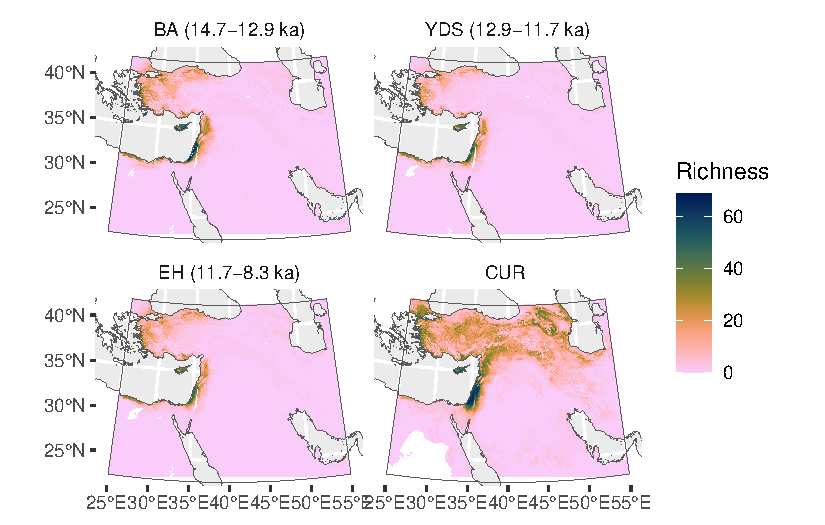
\includegraphics[keepaspectratio]{paper_files/figure-pdf/fig-palaeodist-sum-1.pdf}}

}

\caption{\label{fig-palaeodist-sum}Predicted species richness (sum of
predicted ranges) by period}

\end{figure}%

Many taxa that occur (or are predicted to occur) across the `hilly
flanks' today---including most crop progenitors---are reconstructed to
have had a significantly more restricted distribution in the terminal
Pleistocene/Early Holocene (\textbf{?@fig-sum-palaeodist}). These
include \emph{Ficus carica} (fig); \emph{Hordeum} spp. (wild barleys);
\emph{Lathyrus aphaca} and \emph{L. sativus} (both marginally edible
legumes); \emph{Triticum aestivum compactum} (in the N. Levant),
\emph{T. monococcum aegilopoides}, \emph{T. durum}, and \emph{Triticum
urartu} (but not the other wheat progenitor, \emph{T. turgidum dicoccum}
-- see below); \emph{Aegilops speltoides}, but not \emph{Aegilops
tauschii} (goatgrasses); and \emph{Vicia} spp. (vetches), including
\emph{Vicia faba} (broad beans). most of Anatolia, Northern Mesopotamia,
and the Zagros Mountains in particular disappear from the predicted
ranges of these species, leaving the Levant and to a lesser extent the
Aegean and Cyprus as refugia.

Our results for the Levant are consistent with the current understanding
of this region as developing early intensive foraging economies {[}the
Natufian culture, @{]} and as a centre of origin of agriculture {[}@{]}.
Within the Levant, retreat from the Badia.

Loss of the Northern Mesopotamia--Anatolia region from the predicted
ranges of crop progenitors is interesting in light of the `golden
triangle' hypothesis
\citep{Lev-YadunEtAl2000, KozlowskiAurenche2005, AbboEtAl2010}, which
puts this region at the centre of the development of agriculture.
Multiple lines of archaeological evidence have emerged that point away
from this hypothesis and towards a more geographically diverse origin
\citep{Asouti2006, cites}, but it remains the area with some of the
earliest clear evidence of domestication
\citep{ZoharyHopfWeiss2012, KabukcuEtAl2021, UlasEtAl2024}. Comparative
genetics also points to the Northern Mesopotamia region as the centre of
diversity of many crops \citep[e.g.][]{HaasEtAl2019}. But since these
studies are based on modern genomes, if the wild range of these plants
has, as our modelling suggests, shifted since the Early Holocene, the
apparent centre of diversity may have shifted with them. Our
reconstructions are consistent with the late arrival of intensive
plant-based foraging economies in this region (cf.~the Natufian of the
Levant), and more broadly there need not be a link between the core
\emph{wild} range of a plant and the core area of its domestication. A
scenario in which cultivation emerged at the edges of the ranges of
valuable plant resources---as a means of extend their natural niche---is
also plausible.

The near-absence of the Zagros in any predicted ranges is also
surprising, given mounting evidence that domestication took place just
as early in the eastern \emph{Mashriq} as it did in the west
\citep{Braidwood, GanjDarehGoats, HillyFlanksStuff}. We consider that
the most likely explanation for this is that our flora does not include
the species that were most important to plant subsistence in the east.
Archaeobotanical data on Neolithic sites in the Zagros is limited
(compared to the Levant in particular) due to a hiatus in field research
there from the 1980s to early 2010s \citep{cite}. Recent research
\citep{Amaia} indicates \ldots{}

Cyprus and the Aegean are not conventionally considered part of the
primary zone of domestication but rather amongst the first regions that
acquired agriculture from West Asia. Our analysis complicates this
picture, as it indicates that the wild ranges of many crop progenitors
included these regions. Early examples of several domesticates are
recorded at sites on Cyprus, Western Anatolia and Greece
\citep{ArranzOtaeguiRoe2023}, and the Aegean region was probably
connected to West Asia by a land bridge via Anatolia until the Early
Holocene \citep{AksuHiscott2022}. Were these area part of the same
broader `interaction sphere' \citep{cite} that produce Neolithic
agriculture in West Asia?

Exceptions to the dominant trend of range reduction include \emph{Cicer
reticulatum} (wild chickpea), which has a relatively stable range
centered on Northern Mesopotamia; and \emph{Triticum turgidum dicoccum}
(wild emmer wheat), which is predicted to have two limited ranges
centered around the Black Sea Coast of Anatolia and the Palmyra basin.
In the latter case, neither of these areas are part of the predicted
modern distribution of wild emmer (centered around the Caucasus and
Northern Mesopotamia), but it would be consistent with archaeological
evidence for early cultivation at sites in the Upper Euphrates
\citep{Willcox2024}.

\subsection{Biogeography of crop
progenitors}\label{biogeography-of-crop-progenitors}

\begin{itemize}
\tightlist
\item
  Most cereal and legume crops predicted to be Levantine
\item
  Cereals show diverging southern/northern ranges (legumes not so much)
\item
  Not rye (Anatolia), chickpea (N. Mesopotamia)
\end{itemize}

Wild barley (\emph{Hordeum spontaneum}), its relatives, and pistachio
(\emph{Pistacia atlantica}) show a contraction of their predicted ranges
from the Pleistocene to the Holocene, concurrent with them being brought
into cultivation \textbf{?@fig-palaeodist-barely-pistachio-levant}.
These two species also see marked declines in the archaeobotanical
record from the Early PPNA/Early PPNB (where they were amongst the most
common taxa) to the Late PPNB and Late Neolithic
\citep{ArranzOtaeguiRoe2023}. Conversely, the various wild wheat species
native to West Asia show almost no response to Pleistocene/Holocene
climate change, even within the Levant, and in the archaeobotanical
record wheat displays the opposite trend to barley and pistachio --
becoming gradually more abundant through the course of the Neolithic and
dominant by its end. We hypothesise that climate-linked range shifts
were a factor driving these changes in the apparent economic important
of different crops: the decreasing availability of barley and pistachio
in the terminal Pleistocene may have prompted cultivation as a strategy
to retain access to them, though in the long run it made them less
attractive as staple crops compared to the more resilient wheat.
However, these dynamics are not seen in the majority of crop
progenitors.

The wheat story.

Flax has a very restricted distribution (consistent with low occurrence
in founders paper?). As does Pistacia atlantica, Bolboschoenus maritimus

\emph{Secale cereale} = an Anatolian boy

\subsection{Hindcast models do not predict archaeobotanical
composition}\label{hindcast-models-do-not-predict-archaeobotanical-composition}

The failure of our hindcast models to predict the occurrence of species
in archaeobotanical assemblages has several possible explanations. Since
they do accurately predict the test dataset , a likely culprit is
overfitting of the models to the present environment. This implies that
the modelled palaeodistributions should be seen as conservative
estimates or a minimal range. Another obvious flaw in our methodology is
that the time slices used for palaeoclimatic reconstruction are very
broad---each covering around two millennia---and therefore potentially
unrepresentative of the environment around sites at the specific time at
which they were occupied. The variable quality of the archaeological
test dataset, especially in terms of chronology, is also a plausible
factor.

At the same time, we cannot rule out more substantive reasons for the
discrepency between predicted and observed archaeological occurrences.
The niches of the modelled species could have changed since the Early
Holocene, which would not be captured in a model trained purely on
modern specimens. Human economic choices---mobility, foraging
strategies, cultivation, etc.---could also produce archaeobotanical
assemblages whose composition depart significantly from that of the
surrounding local flora. Further refinement of the methodology for
hindcast palaeoecological niche models, for example using more finely
resolved palaeoclimate sequences \citep[e.g.][]{KargerEtAl2023},
hyperparameter tuning to avoid overfitting, and improved archaeological
datasets, would help disentangle these potential explanations.

Is consistent with more ``macro'' trends such as the reduced range of
Hordeum and Pistacia correlating with its reduced abundance in the
archaeobotanical record.

\section{Conclusion}\label{conclusion}

\begin{itemize}
\tightlist
\item
  We present the first continuous, spatially explicit models of the
  palaeodistributions of N plant species found regularly in association
  with early agricultural archaeological sites in West Asia

  \begin{itemize}
  \tightlist
  \item
    A new line of evidence on archaeoecology
  \item
    Complementary to archaeobot/pollen/etc. because it is independent
    from it
  \item
    All models are wrong\ldots{} but it's easier to see how these are
    wrong than lines on maps
  \end{itemize}
\item
  Modelling at scale using random forest, modern occurrences, and
  hindcasting represents a significant advance in pENM methodology

  \begin{itemize}
  \tightlist
  \item
    Relies on recent open ecological and climatic datasets
  \item
    \ldots open archaeological datasets still lacking!
  \end{itemize}
\item
  First (? - check Yaworsky) attempt to verify hindcast models with
  archaeo. compositional data

  \begin{itemize}
  \tightlist
  \item
    Results not to promising, but this doesn't mean the models are
    useless!
  \item
    Discrepencies suggests several areas for further research and
    methodological development
  \end{itemize}
\end{itemize}


\renewcommand\refname{References}
  \bibliography{references.bib}



\end{document}
